
\documentclass[journal]{IEEEtran}
\IEEEoverridecommandlockouts

\usepackage{fancyhdr}
\usepackage{graphicx}
\usepackage[utf8]{vietnam}
\usepackage{color}
\usepackage{wrapfig}
\usepackage{array}
\usepackage{adjustbox}
\usepackage{nccmath}
\usepackage{subfigure}
\usepackage{amsfonts,latexsym} 
\usepackage{enumerate}
\usepackage{float}
\usepackage{ifpdf}
\usepackage{cite}



\newcolumntype{P}[1]{>{\centering\arraybackslash}p{#1}}  
\newcommand{\tabitem}{~~\llap{\textbullet}~~}
\newcommand{\ctt}{\centering\scriptsize\textbf} 
\newcommand{\dtt}{\scriptsize\textbf} 







\graphicspath{ {Figs/} }  



\newcommand{\MYhead}{\smash{\scriptsize
\hfil\parbox[t][\height][t]{\textwidth}{\centering
\begin{picture}(0,0) \put(-30,-13){\includegraphics[width=50mm]{logo.png}} \end{picture} \hspace{6.4cm}
The University of Information Technology\hspace{5.15cm} Version 1.0\\
\hspace{5.2cm} School of Information and Communication Technology (ICT)\hspace{3cm} \today \\
\underline{\hspace{ \textwidth}}}\hfil\hbox{}}}
\makeatletter

\def\ps@headings{%
\def\@oddhead{\MYhead}
\def\@evenhead{\MYhead}}

\def\ps@IEEEtitlepagestyle{
\def\@oddhead{\MYhead}
\def\@evenhead{\MYhead}}
\makeatother

\pagestyle{headings}

\addtolength{\footskip}{0\baselineskip}
\addtolength{\textheight}{-1\baselineskip}

\begin{document}

\title{Computer Networks and the Internet}

\author{Group 9 - FOBE\\
				\textit{Delay, Loss, and Throughput in Packet-Switched Networks}\\
				Supervisor: Tran Manh Hung\\
} 



\maketitle





\section{Review Questions}	
\subsection*{R18}

Propagation delay:
\begin{equation*} 
    d_{prop} = \frac{d}{s} = \frac{2,500}{2.5 \cdot 10^5} = 10\;ms
\end{equation*}
This delay doesn't depend on packet length and transmission rate ! \\

So, It will take a packet of length 1000\;bytes \textbf{10\;ms} to
propagate over a link of distance 2500\;km.

\subsection*{R19}
\subsection{}
\begin{equation*} 
  \begin{split}
    \text{The throughput for the file transfer} & = min(R1, R2, R3) \\
   & = 500\;kbps
  \end{split}
\end{equation*}
\subsection{}
How long will it take to transfer the file to Host B:
\begin{equation*}
  \begin{split}
  t_{A->B}=\frac{\text{file size}}{\text{throughput for the file transfer}} & = \frac{32000000}{500000} \\
  & = 64\;s
  \end{split}
\end{equation*}

\subsection{}
\begin{equation*} 
  \begin{split}
    \text{The throughput for the file transfer} & = min(R1, R2, R3) \\
   & = 100\;kbps
  \end{split}
\end{equation*}

\begin{equation*}
  \begin{split}
  t_{A->B}=\frac{\text{file size}}{\text{throughput for the file transfer}} & = \frac{32000000}{100000} \\
  & = 320\;s
  \end{split}
\end{equation*}

\section{Problems}


\subsection*{P5}
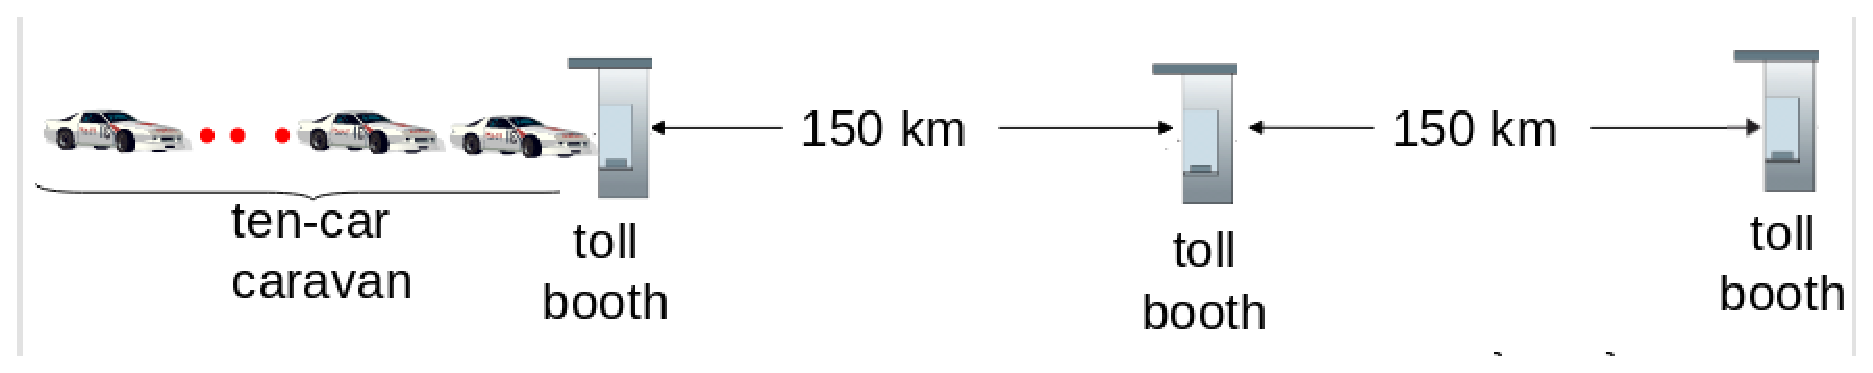
\includegraphics[scale=0.25]{P5}
\subsection{}
The time taken by a car to travel 150\;km:
\begin{equation*}
  \begin{split}
d_{prop}=\frac{\text{distance travelled}}{\text{propagation speed}}  = \frac{150}{100} & = 1.5\;h\\
& = 90\;m
  \end{split}
\end{equation*}
\hspace{0.3cm}The overall tollbooths service time for 10 cars:
\begin{equation*}
  \begin{split}
  d_{trans} = 12 \cdot 3 \cdot 10 & = 360\;s \\
  & = 6\;m
  \end{split}
\end{equation*}
\hspace{0.3cm}End to end delay:
\begin{equation*}
  \begin{split}
  d_{\text{end to end}} = d_{prop} + d_{trans} & = 90 + 6 \\
  & = 96 \;m
  \end{split}
\end{equation*}


\subsection{}
The overall tollbooths service time for 8 cars:
\begin{equation*}
  \begin{split}
  d_{trans} = 12 \cdot 3 \cdot 8 & = 288\;s \\
  & = 4.8\;m
  \end{split}
\end{equation*}
\hspace{0.3cm}End to end delay:
\begin{equation*}
  \begin{split}
  d_{\text{end to end}} = d_{prop} + d_{trans} & = 90 + 4.8 \\
  & = 94.8\;m
  \end{split}
\end{equation*}





\subsection*{P9}
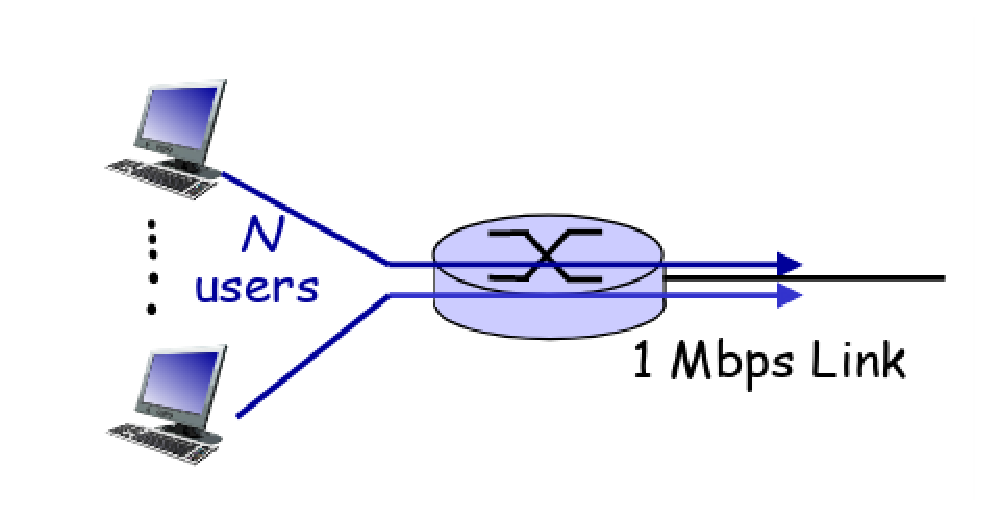
\includegraphics[scale=0.5]{P9}
\subsection*{A.}
The maximum number of users that can be supported simultaneously under circuit switching:
\begin{equation*}
  \begin{split}
    N = \frac{\text{total transmission rate}}{\text{data generation rate of each user }} & = \frac{1 \; Gbps}{1,000 \; kbps} \\
    & = 10,000 \; users
  \end{split}
\end{equation*}

\subsection*{B.}
\hspace{0.3cm}Formula (in terms of p, M,N) for the probability that more than N users are sending data:
\begin{equation*}
  \begin{split}
    P(\text{more than 20 users}) = 1 - \sum_{i=0}^N \binom{M}{i}p^i \; (1-p)^{M-i}
  \end{split}
\end{equation*}




\subsection*{P10}
\begin{figure}[H] 
  \centering  
  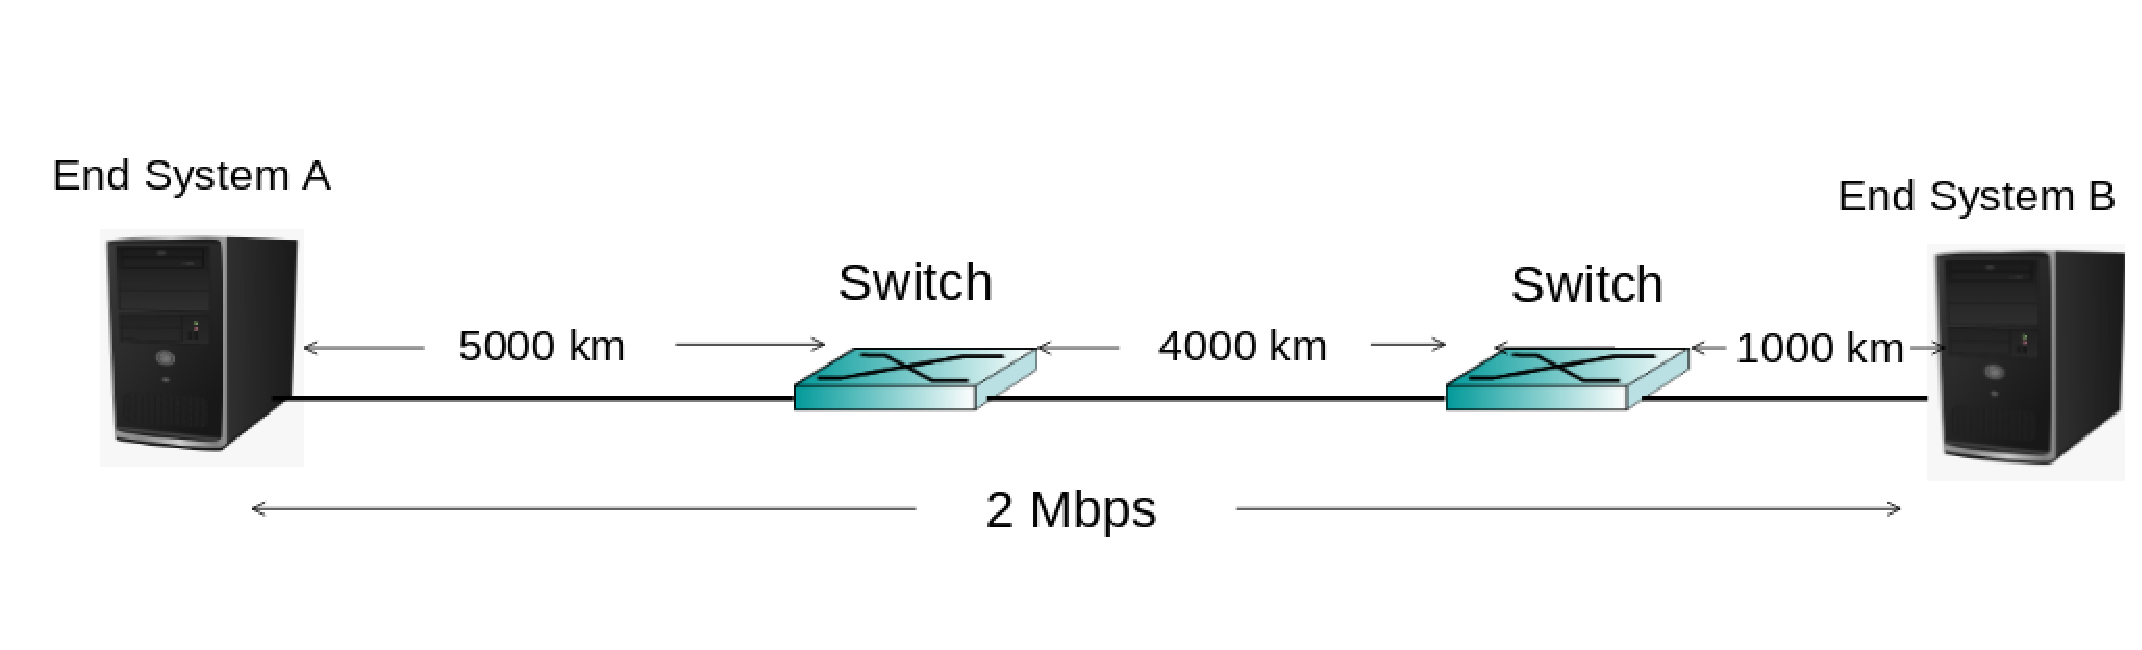
\includegraphics[scale=0.25]{P10} 
  \end{figure}
The packet switch processing delay:
\begin{equation*}
  d_{proc} = 3 \; msec
\end{equation*}
\hspace*{0.3cm} Each link Transmit packet:
\begin{equation*}
  T_{t} = \frac{1,500 \cdot 8}{2 \cdot 10^6} = 0.006 \; s
\end{equation*}
\hspace*{0.3cm} First propagates link:
\begin{equation*}
  d_{prop(1)} = \frac{d_1}{s_1} = \frac{5,000 \cdot 10^3}{2.5 \cdot 10^8} = 0.02 \; s
\end{equation*}

Second propagates link:
\begin{equation*}
  d_{prop(2)} = \frac{d_2}{s_2} = \frac{4,000 \cdot 10^3}{2.5 \cdot 10^8} = 0.016 \; s
\end{equation*}

Third propagates link:
\begin{equation*}
  d_{prop(3)} = \frac{d_3}{s_3} = \frac{1,000 \cdot 10^3}{2.5 \cdot 10^8} = 0.004 \; s
\end{equation*}

End to end Delay:
\begin{equation*}
  \begin{split}
  d & = d_{prop(1)} + d_{prop(2)} + d_{prop(3)} + 2 \; d_{proc} + 3 \; T_t \\
  & = 0.02 + 0.016 + 0.004 + 2 \cdot 0.003 + 3 \cdot 0.004 \\
  & = 0.064 \; s
  \end{split}
\end{equation*}

\subsection*{P12}

\begin{equation*}
  \begin{split}
  \text{Queuing Delay} & = \frac{nL + (L - x)}{R} \\
  & = \frac{8(4 \cdot 1,500 + (1,500 - 750))}{2 \cdot 10^6} \\
  & = \frac{6570 \cdot 8}{2 \cdot 10^6} \\
  & = 0.026 \; s
  \end{split}
\end{equation*}


\end{document}




